\begin{alterendnote}
    这并不是指度量空间.
\end{alterendnote}
\begin{alterendnote}
    ``一篇文章中多一个数学公式, 就会减少一半读者.''
\end{alterendnote}
\begin{alterendnote}
    此处我们认为 $\infty$ 并不是数学分析中由极限所致, 而是一个普通的记号. 诚然其出现会打乱 $\mathbb R$ 的序关系(比如 $\infty +1=\infty$ 等), 但是只要不出现(由于我们舍弃了通过极限达到 $\infty$ 的过程, 因此不可以用任何的极限处理) $\infty-\infty$ 我们都认为结论是没有毛病的.
\end{alterendnote}
\begin{alterendnote}
    此处的 $\mu$ 可以视为来自(measure)的首字母, 或者是可爱猫猫的叫声.
    \begin{center}
        \vskip-\medskipamount
        \label{可爱猫猫}\rotatebox{-5}{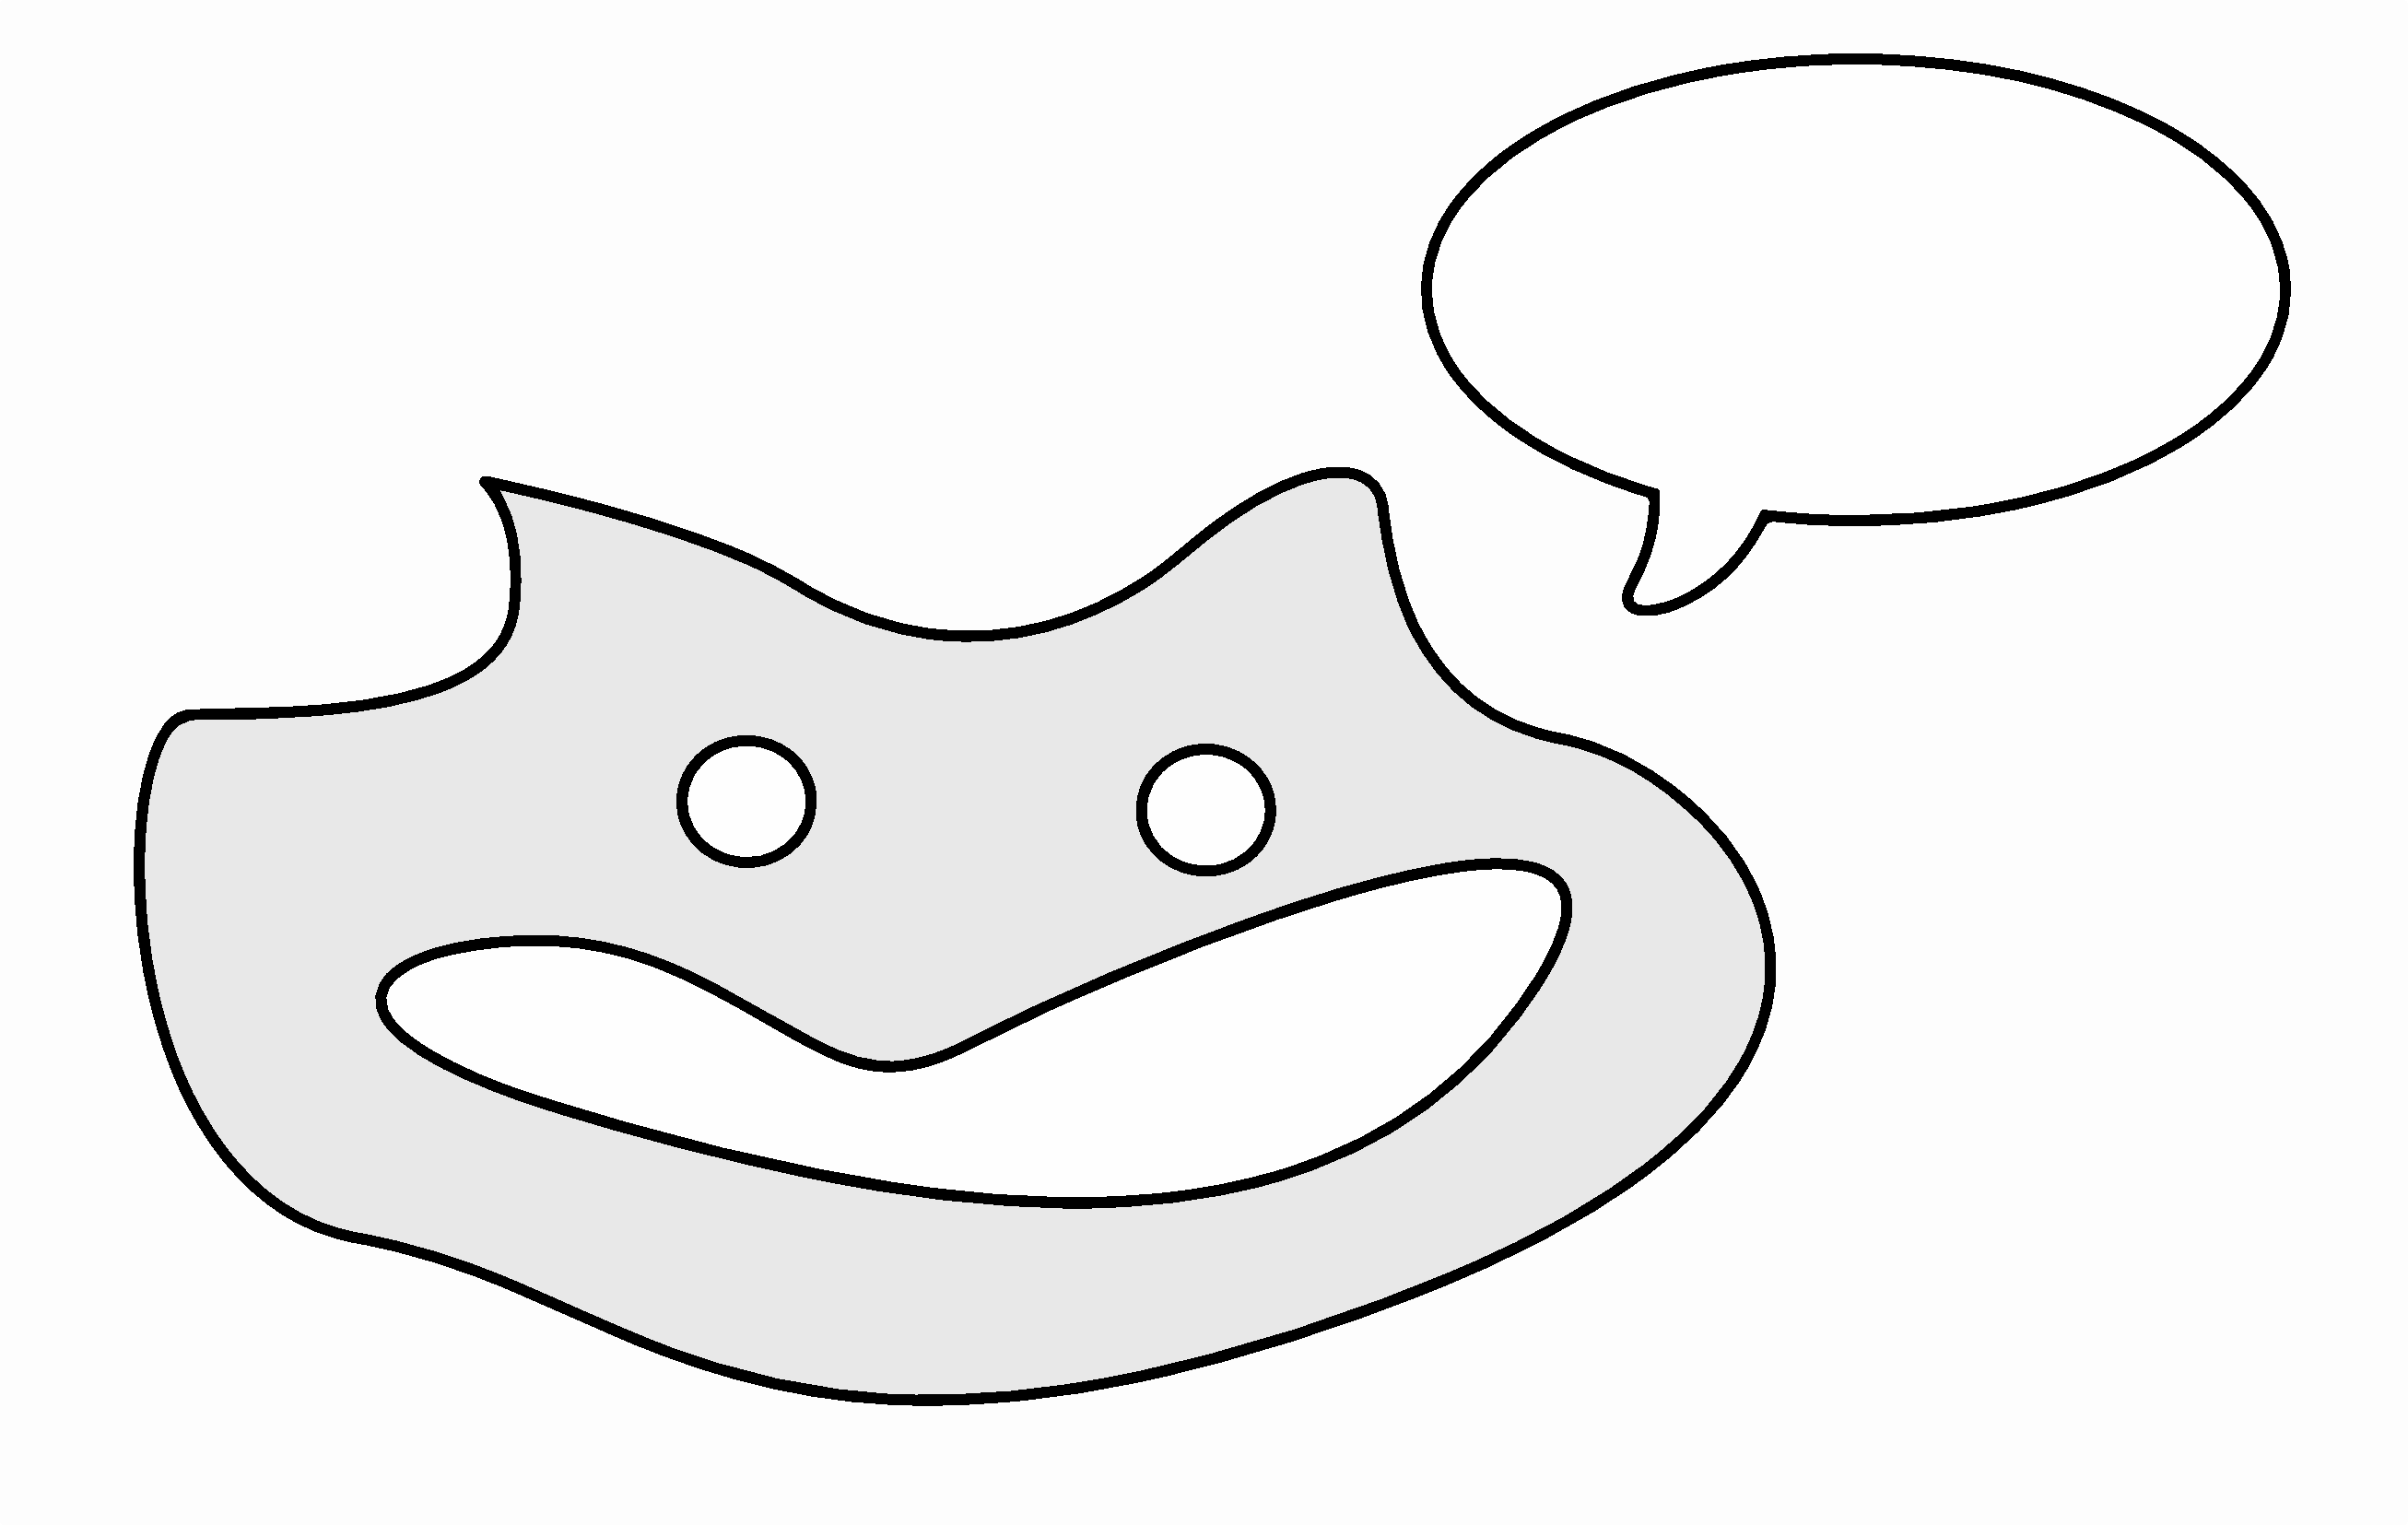
\includegraphics[width=.8\textwidth]{mu.pdf}\raisebox{30.5ex}{\makebox[0pt]{\kern-28ex\Huge\href{https://www.youtube.com/shorts/s9C03DiBU1A}{$\boldsymbol\mu $}}}}
    \end{center}
    \vskip-\medskipamount
    虽然理论上我们用 $m$ 来代表测度更为合适, 但 $m$ 这个记号在 Lebesgue 1902 年的划时代博士论文 \textit{Intégrale, longueur, aire.} 中使用了. 为了纪念他大家以后都会用 $m$ 来表示 Lebesgue 测度.
\end{alterendnote}
\begin{alterendnote}
    S. Banach 本人在此之前得到 $\mathbb R^2$ 和 $\mathbb R$ 并不会产生这种现象: 也即是在 $\mathbb R$, $\mathbb R^2$ 上存在有限可加测度, 且保持平移(旋转)不变性. 但现在观之, 此只能作为一些特例.
\end{alterendnote}
\begin{alterendnote}
    比如``一个半径为 $1$ 的三维球可分成五块并重组成两颗半径为 $1$ 的三维球''. 至于为什么是三维球, 一个有趣的科普可以见 \url{https://www.bilibili.com/video/av2674104/}.
\end{alterendnote}
\begin{alterendnote}
    或者是``物理''.
\end{alterendnote}
\begin{alterendnote}
    你可能会问为什么不用``不可数可加性'', 原因很简单, 因为我们实在是不好处理不可数个数的加法: 在后面我们处理对计数测度的积分(或者用一点点点点拓扑的知识, 用网来将序列极限推广)我们可以一瞥此类求和, 但此与可数情形无异: 求和收敛当且仅当不可数个元素中非零元至多可数, 且该可数求和绝对收敛. 同时, 可数可加性是蕴含有限可加性的, 只需令除了有限个集合外的其他集合为空集即可.
\end{alterendnote}
\begin{alterendnote}
    事实上在第二款中令 $A_n=\varnothing$, 则有``$\mu (\varnothing)=\infty\varnothing \implies \mu (\varnothing)=0$ 或 $\mu (\varnothing)=\infty$.''
\end{alterendnote}
\begin{alterendnote}
    事实上大家都承认.
\end{alterendnote}
\begin{alterendnote}
    为什么是 $\sigma $? 事实上, $\sigma $(或S) 代表德语中的 Summe(求和), 或者对集合的求和(并), 而反之 $\delta $(或D) 来自德语 Durchschnitt(交). 更一般地, 我们用``$\sigma $-''表示可数求和, 比如拓扑空间 $X$ 若是可数个紧集之并, 则称其是\;$\sigma$-紧的.
\end{alterendnote}
\begin{alterendnote}
    当然还有定义在其他结构上的测度, 不过\;$\sigma $-代数是最容易处理的.
\end{alterendnote}
\begin{alterendnote}
    有的书将其称作``可测空间'', 不过这个称呼看上去有点误导性.
\end{alterendnote}
\begin{alterendnote}
    这个定义也不是构造性的, 事实上关于一个子集生成的\;$\sigma $-代数的确有生成公式, 但是并不直观也不好处理. 一个用处是来判断\;$\sigma $-代数的势: 如果 $A$ 到 $\mathbb R$ 有一个单射, 那么 $\mathcal M(A)$ 亦然.
\end{alterendnote}
\begin{alterendnote}
    这类\;$\sigma $-代数的有特殊的作用: 比如说 $X$, $Y$ 是拓扑空间, $f:X\to Y$ 是同胚, 那么我们清楚 $f$ 诱导了 $X$, $Y$ 开集间的一一对应. 同时也诱导了 $\mathcal B_X$, $\mathcal B_Y$ 中集合(称为 Borel 集)的一一对应. 或者, 因为神说``\emph{开集要是可测的}''. 于是就有了 Borel\;$\sigma $-代数. 另外地, 由于还有 Baire $\sigma $-代数, 因此我们有时会记 Borel $\sigma $-代数为 $\mathcal{B}_{\mathrm{orel}}(X)$.
\end{alterendnote}
\begin{alterendnote}
    事实上这种东西叫做拓扑基(或者拓扑子基).
\end{alterendnote}
\begin{alterendnote}
    可数性要求是为了防止我们超出\;$\sigma $-代数只能处理可数交并补的权限.
\end{alterendnote}
\begin{alterendnote}
    一个例子是正项级数求和:对有限个正数求和我们自然可以交换求和顺序, 但对可数个呢? 通过基本的分析学我们知道这也是可以交换的, 即使得到的结果是无穷. 除此之外, 我们还关心非负可积函数列 $\{f_n\}_{n\geqslant 0}$ 会不会有\[\lim_{N \to \infty} \int \sum_{n=0}^N f_n = \int\sum_{n\geqslant 0}f_n.\](即使结果是无穷亦成立, 这看起来有点像二重求和, 虽然我们并不知道 $\sum_{n\geqslant 0} f_n$ 可积性如何), 这其实就是在之后的``单调收敛定理''. 在这种情形下, 将目标分为可数个有限的玩意, 然后分别处理之后加起来也许会有点作用.
\end{alterendnote}
\begin{alterendnote}
    这样看来,\;$\sigma $-有限测度应该叫``半有限测度''更为合适, 但不巧的是半有限测度已经有定义了:若 $E\in\mathcal M$ 且 $\mu (E)=\infty$, 则 $\exists F\subseteq E$, $\infty>\mu (F)>0$. 我们这里不会讨论这种测度.
\end{alterendnote}
\begin{alterendnote}
    如果我们考虑 Dedekind 构造实数的方式, 会发现一个数集的上确界恰好是其对应分划之并.
\end{alterendnote}
\begin{alterendnote}
    如果是拓扑的话, 只考虑序列对应的``连续性''是片面的, 但由于\;$\sigma $-代数只能处理可数次交, 并, 因此考虑序列才能变得自然.
\end{alterendnote}
\begin{alterendnote}
    这个例子来自 Giuseppe Vitali.
\end{alterendnote}
\begin{alterendnote}
    只是一种直观描述而已, 并不是对真正的圆作测度, 在套测度函数之前先把圆拉成线段吧!
\end{alterendnote}
\begin{alterendnote}
    到这里其实就需要用到选择公理.
\end{alterendnote}
\begin{alterendnote}
    事实上 Lebesgue 测度性质比较好, 其零测集的子集必然可测. 这个性质被称为``完备性'', 我们将在\hyperref[外测度与测度的完备化]{第五节}中涉及.
\end{alterendnote}
\begin{alterendnote}
    一个造成其繁琐的原因是我们总有办法让这个零测集子集某种意义上``可测'', 见后文测度完备化的内容.
\end{alterendnote}
\begin{alterendnote}
    事实上, 我们对性质良好的集合可以证明 $\operatorname{inn}\operatorname{area}$, $\operatorname{out}\operatorname{cont}$ 与其的关系: 若 $A$ 是 $\mathbb R^n$ 中的开集, 则 $\operatorname{inn}\operatorname{area}A=A$; 若 $A$ 是 $\mathbb R^n$ 中的紧集, 则 $\operatorname{out}\operatorname{area}A=A$.
\end{alterendnote}
\begin{alterendnote}
    所以它才叫``容度''而不是测度.
\end{alterendnote}
\begin{alterendnote}
    这个例子其实说明 \[D(x)=
        \begin{cases}
            1, & x\in\mathbb Q,    \\
            0, & x\notin\mathbb Q.
        \end{cases}\] 的 Riemann 积分是不存在的.
\end{alterendnote}
\begin{alterendnote}
    和历史的进程一样, Harnack 考虑的``外测度''一开始也只是处理 $\mathbb R$ 上的情形, 我们在这里暂时忽略不单纯的 $\mathbb R^2$, 只处理 $\mathbb R$ 上的情形.
\end{alterendnote}
\begin{alterendnote}
    这里的 $(b_j-a_j)$ 也能换成 $F(b_j)-F(a_j)$, 其中 $F$ 是一个右连续单增函数, 我们管它叫``分布''. 比如令 $F=(\mathord{\arctan} + \pi /2)/2\pi $, 则 $F$ 是一个概率分布. 对于一般的 $F$, 我们管这样子定义的测度(在延拓之后)叫 Lebesgue\,--\,Stieltjes 测度, 直观上来看, 就相当于把 $\mathbb R$ 拉长缩短变形, 而在每点变形(缩涨)的程度刚好是 $F$ 的导数(事实上, $F$ 是几乎处处有导数的, 也就是 $F$ 不可导的点组成一个 Lebesgue 零测集).
\end{alterendnote}
\begin{alterendnote}
    这里考虑 $(a_j,b_j\,]$ 而不是看起来更简单的 $(a_j,b_j)$ 其实是因为 $(a_j,b_j\,]\cup (b_j,c_j\,]  = (a_j,c_j\,]$ 是一个新的半开半闭区间. 而不是像 $(a_j,b_j)\cup (b_j,c_j)$ 这样的中间差了一个点的东西. 事实上如果要考虑在这种中间差了一个点的东西上定义对函数 $F$ 的 Lebesgue\,--\,Stieltjes 测度的话, 势必对 $F$ 的连续性有更高的要求, 这反而是一种束缚.
\end{alterendnote}
\begin{alterendnote}
    为了令 $E\subseteq\bigcup_{j\geqslant 0}A_j$ 的 $A_j$ 选择存在, 我们不妨令 $X\in\mathscr A$.
\end{alterendnote}
\begin{alterendnote}
    除了我们将要探讨的 Lebesgue 测度, 另一个著名的外测度例子是 $\mathbb R^n$ 上的 Hausdorff 测度($\operatorname{diam}$ 是球的直径):\[
        H^s_\delta(E)=\inf\Bigl\{ \,\sum_{j\geqslant 0}(\operatorname{diam}C_j)^s\Bigm| C_j\textit{ 是直径不大于 $\delta $ 的球体},\, E\subseteq\bigcup_{j\geqslant 0}C_k\, \Bigr\}.\]这个测度和分形维数相关, 或者我们可以称为``$s$ 维对应的\;$\delta $-外测度''. 一个例子是 Cantor 集 $C$, 令
    \[
        H^s(C) = \lim_{\delta \to 0^+}H^s_\delta(C).
    \]
    是 $C$ 对应的 $s$ 维 Hausdorff 外测度. 可以证明 $\exists t>0$,
    \[
        H^s(C) = \begin{cases}
            \infty, & s<t, \\
            0,      & s>t.
        \end{cases}
    \]
    我们称 $t$ 为 Cantor 集的 Hausdorff 维数, 可以计算得到 $t = \log 2/\log 3$. 其直观描述大概是:
    \begin{itemize}
        \item 我们用低维的方法去度量高维的集合得到的结果自然是 $\infty$, 用高维的方法度量低维的集合得到的结果自然是 $0$, 对于 Cantor 集这种``有限的集合'', 应该存在一个对应的维度使得其对应度量结果是有限正数.
        \item 注意到我们将 Cantor 集的``直径''缩小为原来的 $1/3$ 得到小 Cantor 集, 两个小 Cantor 集可以拼成一个 Cantor 集. 这个事实有点违反直觉: 缩小为原来的 $1/3$ 得到小 Cantor 集应该要用 $3$ 个才可以拼成原 Cantor 集. 二维平面上的开集``直径''缩小为原来的 $k$ 倍, 则需 $1/k^2$ 个才能拼成原来的开集. ``$^2$''乃是二维所致, 因此类比一下, Cantor 集的对应维数是 $\log _32$. 我们可以将这一过程推广到其他具有严格自相似性质的集合.
    \end{itemize}
    马后炮地说, 我们只是稍稍改了下面积的定义, 在 $s$ 扫过 $[\,0,\infty)$ 的过程中总有一个令其对应测度为有限正数(Hausdorff 维数), 而这个数的大小(当然受限于底空间的维度)可以判别所讨论集合的自相似程度与粗糙性. 更多有趣的内容见 \cite{falconer86}.
\end{alterendnote}
\begin{alterendnote}
    Lebesgue 本人也给出了针对 Lebesgue 测度的可测性条件, 但和 Carathéodory 给出的不同. 事实上 Lebesgue 给出的条件非常依赖于测度的\;$\sigma $-有限性.
\end{alterendnote}
\begin{alterendnote}
    $B$ 当然可以是空集, 故 $\mathcal M\subseteq\overline{\mathcal M}$, 我们在这里跳过这个新结构是\;$\sigma $-代数的证明.
\end{alterendnote}
\begin{alterendnote}
    事实上也只能这样, 按照我们的理解, 零测集的子集必然零测, 故不应该通过并集影响测度.
\end{alterendnote}
\begin{alterendnote}
    事实上单独讨论 $\mathcal B_{\mathbb R}$ 上的测度(Borel 测度) $\mu $ 也会有不少有趣的结果. 在限制测度的有限性的前提下(比如说任意紧集的测度都有限)我们可以给出一个分布:\[F_\mu(x) = \begin{cases}
            -\mu ((x,0\,]), & x<0, \\
            0,              & x=0, \\
            \mu ((0,x\,]),  & x>0.
        \end{cases}\]同时分布可以决定一个 Lebesgue\,--\,Stieltjes 测度.
    \[\mu^F (E)=\inf\Bigl\{ \,\sum_{j\geqslant 0}\bigl(F(b_j)-F(a_j)\bigr)\Bigm| E\subseteq\bigcup_{j\geqslant 0}(a_j,b_j\,]\, \Bigr\}\]
    而此种情况下事实上有 $\mu ^{F_\mu}=\mu $.

    考虑看起来(相比 Lebesgue 测度)不完备的 Borel\;$\sigma $-代数上的测度上的的一个重要性是很多特殊的测度的可测集都包含 $\mathcal B_{\mathbb R}$(毕竟是开集生成的\;$\sigma $-代数), 比如 Lebesgue\,--\,Stieltjes 测度. 而很多与 Lebesgue 测度相关的性质可以同样下放到一般的 Lebesgue\,--\,Stieltjes 测度上. 比如:\[\begin{aligned}
            \mu (E) & =\inf\bigl\{\, \mu (A)\bigm| E\subseteq A,\,A\textit{ 是 $\mathbb R$ 中的开集}\,\bigr\}   \\
                    & = \sup\bigl\{\, \mu (A)\bigm| A\subseteq E,\,A\textit{ 是 $\mathbb R$ 中的紧集}\,\bigr\}.
        \end{aligned}\]
    另外一个有趣例子是 $\lim_{h \to 0} (\mu / m)((x,x+h\,]) = \lim_{h \to 0} (F(x+h)-F(h))/h$ 对应的是 $F$ 的导数(当然对于这样的 $F$ 我们可以要求其不是单增的, 此时就需要考虑符号测度或者复测度). 至于真正处理此类两个测度之比值大概会在 Euclid 空间微分定理相关内容中涉及. 一个经典的例子是: 单调(或有界变差的)函数必然是几乎处处可导的------其隐晦地告诉我们可以将``沿曲线积分''的曲线从方便讨论的分段可微曲线推广成连续可求长曲线. 或者对任何一般的 Lebesgue 可积函数(关于什么是``可积''可以看后文, 事实上这里的可以也可以换成是``局部可积'', 也就是在区间 $[\,a,b\,]$ 上可积), 我们有
    \[
        \lim_{r\to 0} \frac{1}{m(N_r(x))}\int_{N_r(x)} f = f(x),\quad N_r(x) = \{\,y\mid |y-x|<r\,\}
        .\]
    对几乎处处的 $x$ 成立.
\end{alterendnote}
\begin{alterendnote}
    有趣的是这件事并非那么显然, 但的确是从开区间上的性质决定了 $\mathcal L$ 中集合的性质, 这需要用到 Carathéodory 延拓定理, 大概描述的是在描述一个集合(事实上应该是代数)上的测度 $\mu $ 延拓到该集合生成的\;$\sigma $-代数上的测度 $\mu_{\sigma } $ 在 $\mu $ 是\;$\sigma $-有限的前提下, 延拓是唯一的. 故生成的\;$\sigma $-代数可由代数上的测度直接决定. 当然也可以依靠外测度的定义直接证明.
\end{alterendnote}
\begin{alterendnote}
    正所谓``\textit{任何同函数论有关的问题都将导致同集合论有关的某些问题, 只要后面这种问题获得解决或者可能解决, 原有问题就可以随之解决或者近乎解决}.''~------René Baire
\end{alterendnote}
\begin{alterendnote}
    事实上这个记号也有其他意义: $\int_\varnothing \infty$ 应当是 $0$. 但 $\varnothing$ 只是作为最平凡的零测集的例子, 我们想把这个想法延拓到其他零测集上面.
\end{alterendnote}
\begin{alterendnote}
    我们这里不会称为``可积的'', 因为这些函数的积分可能是 $\infty$, 而此种情况我们不会认为函数``可积''.
\end{alterendnote}
\begin{alterendnote}
    事实上我们关注的主要是函数列的上 / 下极限, 上 / 下确界, 因为按我们以前关于\;$\sigma $-代数和测度的处理, 我们只能处理可数个对象.
\end{alterendnote}
\begin{alterendnote}
    我们在这里不写\[\left| \int \psi _n\d \mu-\!\int f\d \mu  \right|\to 0. \]是为了防止 $\infty-\infty$ 的情形.
\end{alterendnote}
\begin{alterendnote}
    自然, 此处用半开半闭区间是为了让我们的分割能首尾相连: 如果用开区间则端点不会被考虑, 用闭区间端点会重复考虑.
\end{alterendnote}
\begin{alterendnote}
    事实上, 与 $f^{-1}([\,a,b\,])$, $f^{-1}((a,b))$, $f^{-1}((a,\infty\,])$, $f^{-1}([\,-\infty,a))$ 可测都等价.
\end{alterendnote}
\begin{alterendnote}
    你可能会想要知道 $\overline{\mathbb R}$ 上的开集是什么, 毕竟是由他们生成了 $\mathcal B_{\overline{\mathbb R}}$. 事实上 $\overline{\mathbb R}$ 就是 $\mathbb R$ 中的开集或者 $\mathbb R$ 中的开集并上 $[\,-\infty,a)$ 或 $(a,\infty\,]$. 一个另一个直观的想法是将 $\overline{\mathbb R}$ 视为是 $[\,0,1\,]$ (比如说复合 $ (\mathord{\arctan} + \pi /2 ) /\pi $), 然后 $[\,0,1\,]$ 上的开集视为 $A\cup [\,0,1\,]$, 其中 $A$ 是 $\mathbb R$ 中的开集.
\end{alterendnote}
\begin{alterendnote}
    如果你要考虑打到 $\mathbb R^n$ 之类的可测函数, 那么定义会稍稍复杂些. 我们此处不处理这些函数.
\end{alterendnote}
\begin{alterendnote}
    另一个暂时性的诠释是, (若读者知晓拓扑的定义的话) $\sigma $-代数和拓扑在某种意义上有些相似: 拓扑应当对有限交与任意并封闭, 而\;$\sigma$-代数对可数交和可数并(以及补)封闭. 事实上, 两个拓扑空间 $(X,\mathcal T)$, $(Y,\mathcal P)$ 间的连续映射 $f:X\to Y$ 应满足\[\forall G\in \mathcal P,\quad f^{-1} (G)\in\mathcal T.\]此与可测空间间的可测函数相对应\[f:(X,\mathcal M_1)\to (Y,\mathcal M_2),\quad \forall A\in\mathcal M_2,\quad f^{-1} (A)\in\mathcal M_1.\]因此广泛点说, 可测函数是保持两个可测空间的\;$\sigma $-代数上结构的映射, 或者称为可测空间组成的范畴之态射, 如同连续映射对拓扑空间, 全纯函数对复空间一般.

    另外地, 看上去\;$\sigma $-代数像是在拓扑的定义上稍作修改, 而我们自然关心这种修改会让其各自对应的``保持结构的映射''改变多少, 也即连续映射与可测映射的关系. 一个著名的定理是 Luzin 定理:
    \begin{theorem}[Luzin]
        对于 $[\,a,b\,]$ 上的可测函数 $f$, 对任意 $\varepsilon>0$, $\exists E_\varepsilon\subset[\,a,b\,]$ 且 $m(E_\varepsilon)<\varepsilon$, $f$ 在 $[\,a,b\,]\setminus E_\varepsilon$ 上连续.
    \end{theorem}
    大概就是我们对拓扑定义的修改所得到对应映射的差异可以被测度控制. 其次, 拓扑中亦有生成的概念:
    \[
        \mathcal T(A) = \textit{包含 $A$ 的最小拓扑} = \bigcap_{T,\textit{拓扑}\atop A\subset T}T,\quad A\subset\mathcal P(X)
        .\]
    不过拓扑的生成与\;$\sigma $-代数的生成有相当大的区别: 最大的区别来自拓扑只要求有限交封闭, 因此我可以让 $A$ 中元素任意有限交得到``原子集合'', 再自由地并起来即可. 因此, 对于拓扑的生成我们有简明的公式
    \[
        \mathcal S(A) = \biggl\{~ G \;\biggm|\; G = \bigcap_{U\in B\atop \mkern-8mu B\subset A,\textit{有限子集}\mkern-8mu} U ~\biggr\},\quad \mathcal T(A) = \biggl\{~ H \;\biggm|\; H = \bigcup_{G\in B\atop B\subset \mathcal S(A)} G ~\biggr\}
        .\]
    或者
    \[
        \mathcal T(A) = \biggl\{~\bigcup_{\textit{任意}}\bigcap_{\textit{有限}} G\;\biggm|\; G\in A  ~\biggr\}
        .\]
    而\;$\sigma $-代数的生成公式则要复杂许多.

    最后一个例子是乘积\;$\sigma $-代数: $\{\mathcal M_ \alpha\}_{\alpha\in A}$ 是\;$\sigma $-代数族, 则乘积\;$\sigma $-代数规定为 $\prod_{\alpha\in A}X_\alpha$ 上令投影映射 $\pi_\alpha$ 可测的最小\;$\sigma $-代数 $\bigotimes_{\alpha\in A}\mathcal M_\alpha$. 因为在前面说过, $\pi_\alpha$ 作为标准的投影映射必然是要保持\;$\sigma $-代数上结构才行, 也即是可测, 而最小\;$\sigma $-代数是因为最大\;$\sigma $-代数 $\mathcal P(\prod_{\alpha\in A}X_\alpha)$ 是平凡的. 一言蔽之:
    \[
        \begin{aligned}
            \pi_\alpha \textit{ 可测} & \implies E_\alpha\in\mathcal M_\alpha, \quad\pi _\alpha^{-1} (E_\alpha) \in \bigotimes_{\alpha\in A}\mathcal M_\alpha                                               \\
                                      & \implies \bigotimes_{\alpha\in A}\mathcal M_\alpha = \mathcal M( \{\, \pi _\alpha^{-1} (E_\alpha) \mid E_\alpha\in \mathcal M_\alpha,\,\forall \alpha\in A\, \}  ).
        \end{aligned}
    \]
    而此与乘积拓扑 $\mathcal T (\{\,\bigcap_{\alpha\in B\atop B\subset A,\textit{有限子集}\mkern-8mu} \pi _\alpha^{-1} (E_\alpha) \mid E_\alpha~\textit{是}~X_\alpha \textit{ 中开集}\,\})$ 的构造不谋而合. 乘积\;$\sigma $-代数的一个作用是讨论 $\mathbb R^n$ 中的 Lebesgue 可测集, 事实上 $\mathcal L^n = \overline{\prod_{j=1}^n\mathcal L}$. 也即是在 $\mathbb R$ 的 Lebesgue 可测集乘积 $n$ 次后的完备化, 至于其对应的 Lebesgue 测度, 可由在矩形上的处理 $m^n(\prod_{j=1}^n (a_j,b_j\,]) = \prod_{j=1}^n(b_j-a_j)$ 延拓至 $\overline{\prod_{j=1}^n\mathcal L}$ 得到(事实上我们当然可以一步到位直接延拓到最大的那个\;$\sigma $-代数, 但考虑乘积拓扑可以通过完备化的方式让我们对可测集的构造有更深的理解, 因此\hyperref[AcupN]{正规性}对 $\mathbb R^n$ 中的 Lebesgue 测度也是成立的).

    至于为什么说这个诠释是暂时性的, 事实上我们可以在远弱于\;$\sigma $-代数的结构上定义测度(比如半环), 而这些结构其实与拓扑差距甚大, 因此与拓扑的类比作为引入用的暂时性例子是更合适的.
\end{alterendnote}
\begin{alterendnote}
    这里的 $L$ 其实是为了纪念 Lebesgue, 即使我们并没有处理 Lebesgue 测度.
\end{alterendnote}
\begin{alterendnote}
    其实对广义的 Riemann 积分非也, 考虑 $f(x)=\sin x /x$, 则其在 $(0,\infty)$ 上的 Lebesgue 积分不存在, 而广义黎曼积分为 $\pi /2$. 所以在某种意义上, 不绝对可积的函数就是不可积函数.
\end{alterendnote}
\begin{alterendnote}
    回忆一下我们断言对测度的积分可以将各式各样的求和统一在一起, 我们不妨用计数测度的语言来说明一下单调收敛定理和控制收敛定理:
    \begin{theorem}[单调收敛定理]
        令 $\{a_{nm}\}_{n,m\geqslant 0}$ 是正项序列, 则
        \[
            \sum_{n\geqslant 0}\sum_{m\geqslant 0}a_{nm} = \sum_{m\geqslant 0}\sum_{n\geqslant 0}a_{nm}
            .\]
        允许求和值为 $\infty$ 的情形.
    \end{theorem}
    \begin{theorem}[控制收敛定理]
        令 $\{a_{nm}\}_{n,m\geqslant 0}$ 是复数序列, 且满足 $\lim_{n \to \infty} a_{nm} = A_m$. 若
        \[
            \sum_{m\geqslant 0}\Bigl(\sup_{n\geqslant 0} |a_{nm}|\Bigr) <\infty
            .\]
        则
        \[
            \lim_{n \to \infty}\sum_{m\geqslant 0}a_{nm} = \sum_{m\geqslant 0}A_m < \infty
            .\]
    \end{theorem}
\end{alterendnote}
\begin{alterendnote}
    事实上, Riemann 积分中也有相似的控制收敛定理:
    \begin{theorem}
        $\{f_n\}_{n\geqslant 0}$ 是定义在 $[\,0,\infty)$ 上的函数列, 且在 $\forall[\,a,b\,]\subseteq[\,0,\infty)$ 上 Riemann 可积, 且 $f_n\to f$, 其中 $f$ 在 $\forall[\,a,b\,]\subseteq[\,0,\infty)$ Riemann 可积, 若存在 Riemann 可积函数 $g$ 满足 $|f_n|\leqslant g$ 对任意 $n$ 成立, 且 $\int_{[0,\infty)}g<\infty$, 则  \[\lim_{n \to \infty} \int_{[0,\infty)} f_n = \int_{[0,\infty)} f.\]
    \end{theorem}
    \noindent 有关这个定理的细节可以参考\cite{Cunningham67} (事实上这个定理也可以通过 Lebesgue 测度下的控制收敛定理马后炮地推出来).
\end{alterendnote}
\begin{alterendnote}
    也就是\[\nu (E)=\inf\Bigl\{ \,\sum_{j\geqslant 0}\bigl(F(a_j)-F(b_j)\bigr)\Bigm| E\subseteq\bigcup_{j\geqslant 0}(a_j,b_j\,]\, \Bigr\}\]其中 $F$ 是单增右连续函数.
\end{alterendnote}
\begin{alterendnote}
    事实上, 这样的 $f$ 并不是唯一的, $f$ 自然可以在一个\;$\mu $-零测集下乱跑, 只需保证是可测的即可. 同时, 由于 $\nu $ 和 $\mu $ 都是非负的, 因此 $f$ 也是几乎处处非负的, 若要考虑 $\mathbb R$ 甚至 $\mathbb C$ 上的函数, 则须引入符号测度或复测度.
\end{alterendnote}
\begin{alterendnote}
    事实上, Radon\,--\,Nikodym 定理阐明, 如果 $\nu$ 对 $\mu $ 绝对连续, 其中 $\nu$ 可以是一般的(正)测度, 也可以是符号测度或者复测度, $\mu $ 是正测度, 且两个测度都是\;$\sigma $-有限的, 且定义在同一个\;$\sigma $-代数上. 那么满足
    \[
        \nu (E) = \int_E f\d \mu
        .\]
    的 $f$ 必然存在, 且在相差一个\;$\mu $-零测集的情形下唯一.
\end{alterendnote}
\begin{alterendnote}
    事实上这个奇特的``测度的绝对连续''定义与函数的绝对连续之间有强烈的关联: 对于一个右连续有界变差函数 $F$(且满足 $\lim_{x\to -\infty}F(x) = 0$), 其生成的 Lebesgue\,--\,Stieltjes 测度 $\mu ^F$ 对 Lebesgue 测度绝对连续当且仅当 $F$ 在 $\mathbb R$ 上绝对连续. 至于什么是有界变差, 其实我们考虑一个(可以是不单调的)右连续函数生成的 Lebesgue\,--\,Stieltjes 测度. 我们(自然)希望有
    \[
        \begin{aligned}
            \mu ^F((a,b\,]) & = \sum_{n\geqslant 0}\mu ^F((x_n,x_{n+1}\,])                                                         \\
                            & = \sum_{n\geqslant 0}(F(x_{n+1})-F(x_n)),    & \quad a=x_0<x_1<x_2\cdots <\lim_{n \to \infty} x_n=b. \\
        \end{aligned}
    \]
    是绝对收敛的(更好的情形是无论如何选取 $\{x_n\}_{n\geqslant 0}$, $\sum_{n\geqslant 0}|F(x_{n+1})-F(x_n)|$ 总是有一个共同上界). 因为这个求和本来就不应该与我们的求和顺序相关(由于 Riemann 重排定理, 条件收敛的级数可以通过重排收敛到任何值). 因此我们有了以下要求:
    \[
        \mathop{\vcenter{\hbox{\LARGE$\mathbf{V}$}}}_{[a,b]}F \coloneqq \sup_{n\geqslant 0}\biggl\{\,\sum_{j=0}^n|F(x_{j+1})-F(x_j)|\biggm|a=x_0<x_1<\cdots <x_n=b\,\biggr\} < \infty
        .\]
    此时称 $F$ 是 $[\,a,b\,]$ 上的有界变差函数. 另外地, 选取这个定义还与曲线的长度相关: 若 $F:[\,a,b\,]\to \mathbb C$, 则 $\mathop{\vcenter{\hbox{\Large$\mathbf{V}$}}}_{[a,b]}F$ 实际上是 $\operatorname{im}F$ 的长度.
    
    粗略地来说, 有界变差是对可求长曲线的推广, 也是对单调函数的推广(因为有界的单调函数必然是有界变差的, 事实上, 打到 $\mathbb R$ 上的有界变差函数可以写为两个单增函数之差). 在之前的注记中提到过, 有界变差函数几乎处处有导数, 因此对于可求长曲线, 其切向量几乎处处存在, 这让沿着可求长曲线的积分称为了可能.
    
    有趣的是, 有界变差的定义并非来自对测度的处理, 事实上, 有界变差要求 $F$ 在局部的振幅不应过大, 而 Fourier 级数的收敛亦与振幅直接相关. 事实上, Jordan 在 1881 年的一篇论文 \emph{Sur la série de Fourier} 中引入了这个概念.
    
    回到对单调函数的讨论中来. 我们可以对单调(递增)函数作以下著名的分解:
    \[f = f_{\mathrm D} + f_{\mathrm{AC}} + f_{\mathrm{SC}}.\]
    其中三者都有独特的性质:
    \begin{itemize}
        \item $f_{\mathrm D}$ 是一个``离散(Discrete)''的函数: $\sum_{n\geqslant 0}a_n\chi_{\{b_n\}}$, 其实代表着 $f$ 的不连续点, 减去这些不连续点所造成的差之后 $f$ 就连续了;
        \item $f_{\mathrm{AC}}$ 可以求导, 且满足微积分基本定理: \[\int_a^b f_{\mathrm{AC}}' = f_{\mathrm{AC}}(b)-f_{\mathrm{AC}}(a).\] 根据微积分基本定理我们知晓此时 $f_{\mathrm{AC}}$ 绝对连续(Absolutely Continuous);
        \item $f_{\mathrm{SC}}$ 比较特殊, 其对应的是``导数几乎处处为 $0$ 但是并不是常数函数''的函数. 事实上, 由 Fatou 引理我们可以得到: \[f(b) - f(a) \geqslant \int_{a}^b f'.\] 而 $f_{\mathrm{SC}}$ 就是其中 $f(b) - f(a) > \int_{a}^b f'$ 的那一部分. 此时 $f_{\mathrm{SC}}$ 是奇异连续(Singular Continuous)的. 一些不太雅观的例子就像是``严格单增但导数几乎处处为 $0$'' 的连续函数一样(见\cite{Brown69}).
    \end{itemize}
    由于一般的有界变差函数可以由单调函数拼成, 因此这个分解也可以对一般的有界变差函数有效, 在某种意义上这属于我们对一个有界变差函数分解的最终情形.
\end{alterendnote}
\begin{alterendnote}
    \label{Fubini}事实上, 这个结果也可以推广到一般的\;$\sigma $-有限测度. \par 说点题外话, 读者会发现我们列举的许多定理都要求\;$\sigma $-有限测度, 事实上在这些定理的经典证明中, 往往都是先对有限测度讨论, 然后再通过可数相加推广到\;$\sigma $-有限测度.\;$\sigma $-有限测度最著名的例子当然是 Lebesgue 测度, 非\;$\sigma $-有限测度的典例当属不可数集上的计数测度. 因此某种意义上, 计数测度虽然看起来简单, 但却与某些反例息息相关. 至于有限测度有什么优点\,$\mathinner{\ldotp \ldotp \ldotp\ldotp \ldotp \ldotp}$\,我想最直观的应当是对集列下降情形的连续性 \hyperref[测度的连续性:集列下降]{(点这儿!)}.
\end{alterendnote}
\begin{alterendnote}
    Fubini\,--\,Tonelli 定理看似只是处理普通的积分换序问题------很容易和多元微积分中的 Fubini 定理类比, 但正如边注 \ref{Fubini} 所说的, Fubini\,--\,Tonelli 定理可以推广到\;$\sigma $-有限测度的情形: 比如可数集上的计数测度.
    \begin{theorem}[Fubini, Tonelli]
        令 $f$ 是测度空间 $(X,\mathcal M)$ 上的可测函数, $\mu _1$, $\dots $, $\mu _n$ 是定义在 $\mathcal M$ 上的\;$\sigma $-有限测度, 则:

        若 $f\geqslant 0$ 或 $f\in L(\mu_1 \times \cdots \times \mu _n)$, 则
        \[
            \int f \d (\mu_1\times \cdots \times \mu _n) = \int\left(\,\cdots \!\int\left(\, \int f \d \mu_1 \right) \d \mu_2\cdots \right)\d \mu_n
            .\]
    \end{theorem}
    考虑可数集上的计数测度如下:
    \begin{theorem}
        令 $\{\,f_n: \mathbb R^d\to \mathbb C\,\}_{n\geqslant 0}$ 是可测函数列, 则若 $\sum_{n\geqslant 0}\int |f_n|\d m^d<\infty$, 则
        \[
            \sum_{n\geqslant 0}\biggl(\int f_n\d m^d\biggr) = \int_{\mathbb R^n}\biggl(\,\sum_{n\geqslant 0} f_n\d m^d\biggr)
            .\]
    \end{theorem}
\end{alterendnote}
\begin{alterendnote}
    在这之中有一个看起来相当麻烦的问题: 事实上$\int f(x_1,\dots,x_n)\d x_1$可能并不是对所有的$(x_2,\dots,x_n)$都是可测的, 我们只能证明其对几乎处处的 $(x_2,\dots,x_n)$ 都可测, 因此我们必然要考虑这个函数在一个零测集上面是没有定义的. 由于是零测集(事实上还依赖于 Lebesgue 测度的完备性), 我们不妨把没有定义的地方补 $0$ 以便继续积分. 用看起来比较高级点的语言来说就是我们是对``函数的等价类''进行积分, 这些函数几乎处处有定义, 且两个函数等价当且仅当他们在定义域交集内相等.
\end{alterendnote}
